\section{Signal-to-noise ratio}
In this section the term SNR introduced in chapter \ref{ch10} is described, and it is further used to analyze the additive noise on the recorded audio.
SNR is a measure of the amount of noise in a signal. 
The SNR is defined as
\begin{align} \label{eq:SNR}
	SNR=\frac{\sigma_{signal}^2}{\sigma_{noise}^2},
\end{align}
where $\sigma_{signal}^2$ is the variance of the wanted signal, and $\sigma_{noise}^2$ is the variance of the noise \cite{page 228, DTSP}.

To try and determine how small the SNR is allowed to be the recorded music will be added noise in various level such that the SNR gradually changes.
The peak detection algorithm is then used to find peaks, and it is observed when it does no longer manage to find the right peak as a consequence of the excessive noise in the signal.

To calculate the variance $\sigma^2$ of the signal and noise the standard deviation $\sigma$ of the signal can be calculated. 
If the input signal is zero mean, the standard deviation of the signal can be calculated by the root mean scare of the signal \cite{page 228, DTSP}.

The root mean scare (RMS) is defined as
\begin{align*}
	x_{rms} 
	&=\sqrt{\dfrac{1}{n} \sum_{i=1}^n x_i^2}\\
	&= \sqrt{\dfrac{x_1^2 + x_2^2 + \dots + x_n^2}{n}},
\end{align*}
where $\sigma = x_{rms}$ in the previous mentioned instance with zero mean. An algorithm calculating the SNR of the audio signal is implemented in Python.

\section{Varying signal-to-noise ratios}
To measure the varying amount noise in the signal the SNR as defined in definition \ref{def:SNR} is used. The peak detection alogrithm will be tested by gradually increasing the amount of noise in the signal and thereby decreasing the SNR of the signal. The evaluation of the peak detection alogrithm is then based upon the SNR at the time of failure of the algorithm.

\subsection{Single tone}
The signal of a single tone is added the noise of clapping, singing, folding a piece of paper and ambient noise in varying levels. Figure \ref{fig:single_spectrum} shows the frequency spectrum of the signal, the noise signal and the bandpass filter.

\begin{figure}[H]
\begin{subfigure}{0.49\textwidth}
\centering
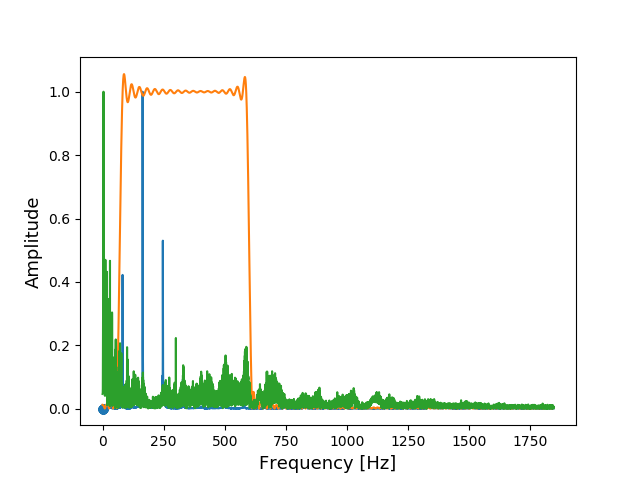
\includegraphics[width=\textwidth]{figures/SNR/single_spectrum.png}
\caption{Normalized frequency spectra of single low $E$ tone (blue), the noise signal (green) and the bandpass filter (orange).}
\label{fig:single_spectrum}
\end{subfigure}
\begin{subfigure}{0.49\textwidth}
\centering
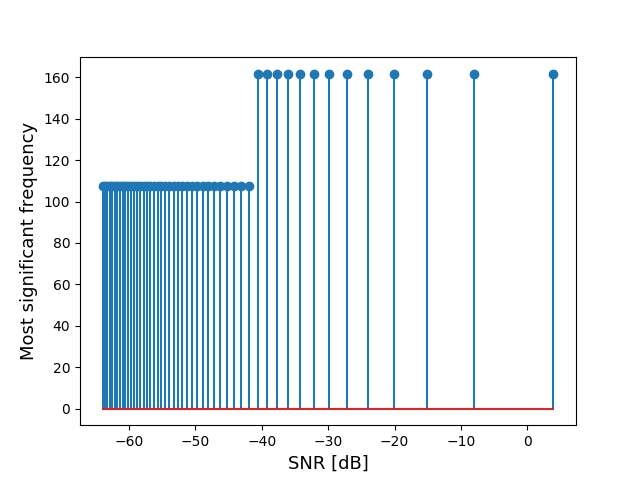
\includegraphics[width=\textwidth]{figures/SNR/single_stem.png}
\caption{Stem plot of most significant frequencies of noisy signal at different levels of SNR.}
\label{fig:single_stem}
\end{subfigure}
\caption{}
\label{fig:single_noise}
\end{figure}

The noise-free signal has a most significant frequency of 167.58 Hz corresponding approximately to a harmonic of an $E$ tone. By letting the SNR decrease and running the peak detection algorithm at each step of different SNRs the stem plot of most significant frequencies in figure \ref{fig:single_stem} is created. This plot shows when the peak detection fails to identify the most significant frequency in the signal. At SNR = -37.83 dB the peak detection algorithm no longer detects the right frequency but another frequency of 105.84 Hz which is assumed to be the most significant frequency of the noise added to the signal.

\subsection{White noise}
A generated sampling of white noise is furthermore added to the single tone. Figure \ref{fig:white_spectrum} shows the frequency spectra of the signal, noise and filter.

\begin{figure}[H]
\begin{subfigure}{0.49\textwidth}
\centering
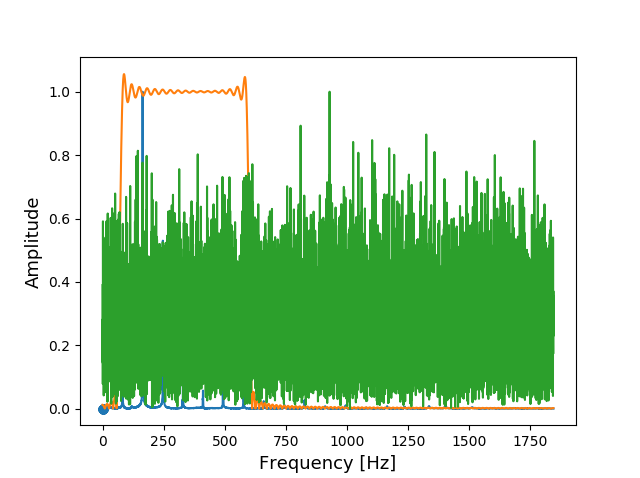
\includegraphics[width=\textwidth]{figures/SNR/white_spectrum.png}
\caption{Normalized frequency spectra of single low $E$ tone (blue), white noise (green) and bandpass filter (orange).}
\label{fig:white_spectrum}
\end{subfigure}
\begin{subfigure}{0.49\textwidth}
\centering
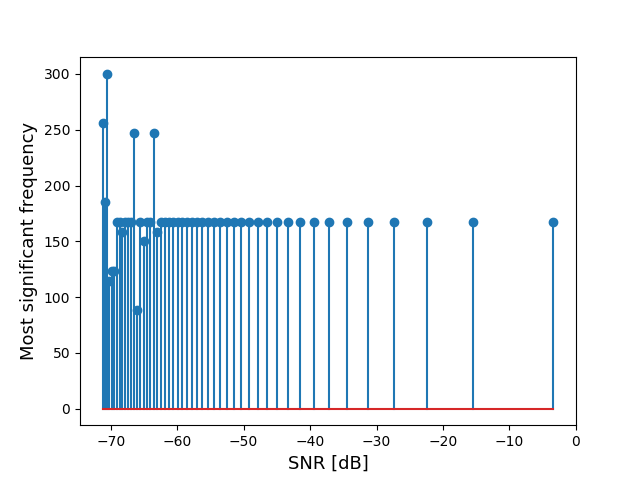
\includegraphics[width=\textwidth]{figures/SNR/white_stem.png}
\caption{Stem plot of most significant frequencies of noisy signal at different levels of SNR.}
\label{fig:white_stem}
\end{subfigure}
\caption{}
\label{fig:white_noise}
\end{figure}

In figure \ref{fig:white_stem} it is seen that the peak detection algorithm no longer detects the right frequency from SNR = -62.46 dB but rather detects random frequencies as a result of the overwhelming amount of white noise.

\subsection{Concentrated noise}
Figure \ref{fig:concentrated_noise} shows the results of adding noise concentrated in a single frequency in the passband to the signal. Concentrating the power of the noise in a single frequency of 300 Hz bypasses the filter and is easily detected by the algorithm.

\begin{figure}[H]
\begin{subfigure}{0.49\textwidth}
\centering
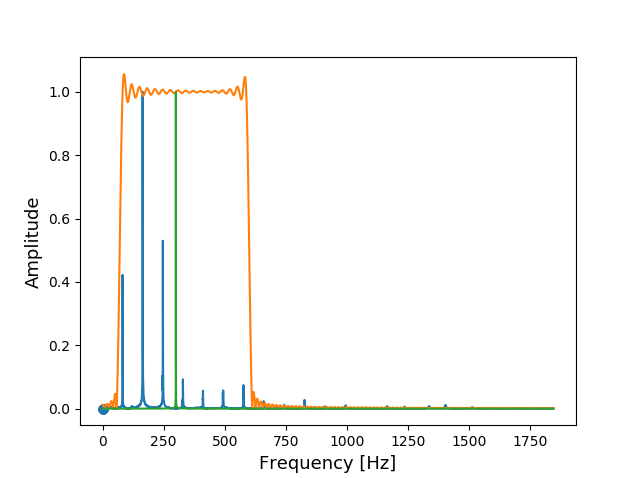
\includegraphics[width=\textwidth]{figures/SNR/concentrated_spectrum.png}
\caption{Normalized frequency spectra of single low E tone (blue), concentrated noise at 300 Hz (green) and bandpass filter (orange)}
\label{fig:concentrated_spectrum}
\end{subfigure}
\begin{subfigure}{0.49\textwidth}
\centering
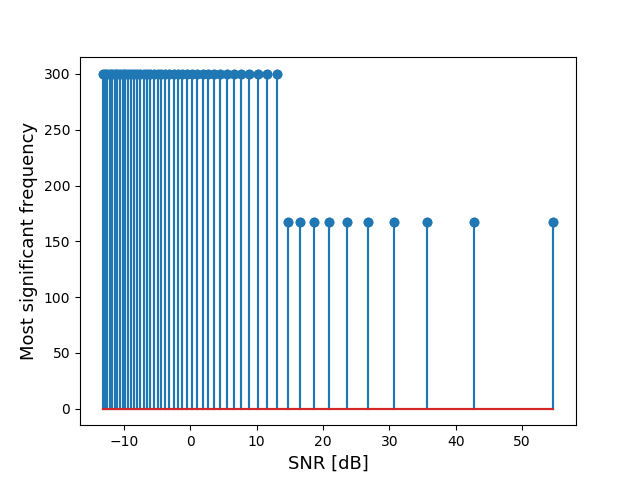
\includegraphics[width=\textwidth]{figures/SNR/concentrated_stem.png}
\caption{Stem plot of most significant frequencies of noisy signal at different levels of SNR.}
\label{fig:concentrated_stem}
\end{subfigure}
\caption{}
\label{fig:concentrated_noise}
\end{figure}

As seen in figure \ref{fig:concentrated_stem} the peak detection algorithm no longer detects the right frequency at SNR = 13.06 dB. This is in stark contrast with the two above simulations and is because of the concentrated energy in a single frequency lying in the passband.

\section{Summary}
From the above tests of the peak detection algorithm under varying amounts of different noise the following three points can be made:
\begin{itemize}
\item If the energy in the noise signal lies outside the frequency band it is filtered out by the band pass filter.
\item If the noise lies in the pass band but the energy is spread in different frequencies the algorithm works well.
\item If the noise lies in the pass band and the energy is concentrated in few frequencies the algorithm does not work well.
\end{itemize}
For the purpose of the algorithm in this project - filtering background noise - the algorithm is concluded to work well as it can detect peaks at very low levels of SNR.